
%quantitative-fvr experiments
%stereo-
%fvr-sota
%mvvdscfds%%%r
%qual
%

In order to quantitatively compare and analyse the FVR, FFVR, FVR-3D and MVVR extensions, several real world data were used to study its potential in conjunction with 3 sensor types: stereo, active camera and monocular camera. These data all contain full RGB color information as well as 3D structural information per frame. In the case of stereo this data is taken from ground truth laser scans. This is done to simulate the ideal high quality and dense 3D data which may be computed by stereo camera set-ups and disparity calculation algorithms. In the case of active camera data, the 3D structural information is taken directly from the Asus Xtion PRO live camera. In monocular tests, depth information is computed between frames using techniques from disparity computation and optical flow based methods. \\ 

To assess qualitative reconstruction, three scenes were captured and registered using the FVR method. These scenes include the apartment scene, office scene and the garden scene. All three scenes were captured using the Asus XTION PRO live active camera at 30 frames per second. For each scene, only one in every 30 frames were registered, constituting real time FVR performance. The apartment scene was generated by moving and rotating the camera around an apartment living room before moving towards the kitchen area. This scene contains an abundance of features and would be considered a basic test for most 3D reconstruction algorithms. The second scene is the Office scene. This scene was generated by rotating the camera whilst zooming in and out on different objects within the room. Again this scene was reconstructed by registering every 30th frame. Despite both of the scenes being trivial to reconstruct, most algorithms (especially feature matching based methods) would find registering large rotations (such as those present in this data) difficult. The Garden scene is a difficult scene to reconstruct regardless of the reconstruction algorithm or technique used for registration. This scene was captured by rotating the camera around a garden outside the university. The scene contains many textures which are similar at the local level but are located in totally different locations. Therefore the scene is difficult to reconstruct using local and feature based methods such as FM+RANSAC and ICP. \\


 

%mark for removal
To analyse the robustness of the FVR method in terms of camera translation and rotation an indoor environment was captured using the Asus Xtion PRO live active camera. The results and descriptions for these experiments are shown in sections \ref{Sec:CamTransTrackExp} and \ref{Sec:CamRoteTrackExp}. This indoor environment contained several boxes and pieces of furniture. Therefore the data provide a useful and challenging but robust test for this 3D reconstruction method. The robustness of the FVR method in situations where moving objects impact registration is measured. Several 3D frames were captured for this experiment. These frames are captured from an indoor scene where furniture of different sizes are removed and added between frames. \\



The MVVR method was analysed using test data generated using a Microsoft passive RGB camera. The data output is in basic video format, and all depth information was generated implicitly by the MVVR algorithm. This data was captured by moving the camera whilst focusing on a set of textured boxes within an indoor environment. Several frames were captured at 30 frames per second and registered for analysis of the MVVR method qualitatively. Quantitative tests of the MVVR make use of the same data as tests for the FVR method (testing translation and rotational registration error). \\

Test data was also generated in order to robustly test and compare the FVR series of methods proposed in this research with different pose-estimation procedures and 3D registration methods in a variety of different scenes and settings each with features which push the boundaries for reconstruction in some way. Scenes which are both in-door and out-door were chosen for testing in order to measure the robustness and accuracy of these methods in both settings. Some scenes include large amounts of texture whilst others have little or no texture. Scenes with little texture are difficult for both SLAM and 3D reconstruction techniques because of the small amount of usable data by which a registration may be computed. Some scenes in the data-set were captured purposefully to measure the accuracy of these algorithms when large amounts of local features are identical within the scene. These scenes may confuse local methods because they contain multiple items/features/image patches which look similar locally but are actually different parts of possibly different objects within the scene, each having a unique global position which may be distant from that of another similar feature. Such scenes include carpet, plant-life, grass and generic plane walls or tiles. \\

This test-data also measures the accuracy, robustness and usefulness of each algorithm to register camera movements of different types. Each scene is captured with the camera performing certain an often singular type of movement. By testing with different movements, future algorithms may be constructed by switching to different registration methods based on camera movement. The different camera transformations recorded in the test data include: translation (left and right), zooming (and moving forward/backward) and rotation about different axes (x and y axis). \\

Some frames from these test videos are shown in appendix \ref{AppendixA}. The first scene: the Apartment Texture Rotate scene was taken by rotating the camera around the y-axis across an apartment. This scene contains a lot of texture information. The Apartment Texture X Axis scene is similar in terms of texture but contains both x and y axis rotation. This tests the FVR's ability to handle multiple axes of rotation. \\


The boxes scene was captured under arbitrary-rotation, translation and zoom (in/out) camera motions. It contains some useful information on the boxes themselves, however the texture on the carpet may cause texture confusion for feature based registration methods. The Desk Texture Translation scene contains a desk with a desktop computer and several items on it. The In-door space with texture-confusion contains a set of chairs and picture frames which look similar to each-other locally but may cause confusion for registration techniques which rely on local features. \\

The kitchen scene was captured with both translation and zoom camera movements. It contains very little texture with most of the scene containing a plain/flat white textured surface. The Office textured blind-spot rotation scene is a textured office scene where the camera is rotated about the y-axis. The scene is focused on a large divider which separates two desks. The divider may confuse registration methods which rely too heavily on minimization by aligning the large divider as a priority rather than taking into account the smaller details within the scene. An example of such an algorithm would be ICP and its derivatives. \\

The Office scenes contain a plenty of usable texture and different sets were created by translating, rotating about the y-axis and rotating about the x-axis. Other office scenes, where the camera captures objects in both the foreground and the background and where the camera is lifted and rotated whilst focussed on an office desk and chair combo. Some out-door scenes were also captured around the university. They are captured with both rotation and translation camera movements and are also labelled as being susceptible to texture confusion. \\

\begin{figure}[!htb]
\centering
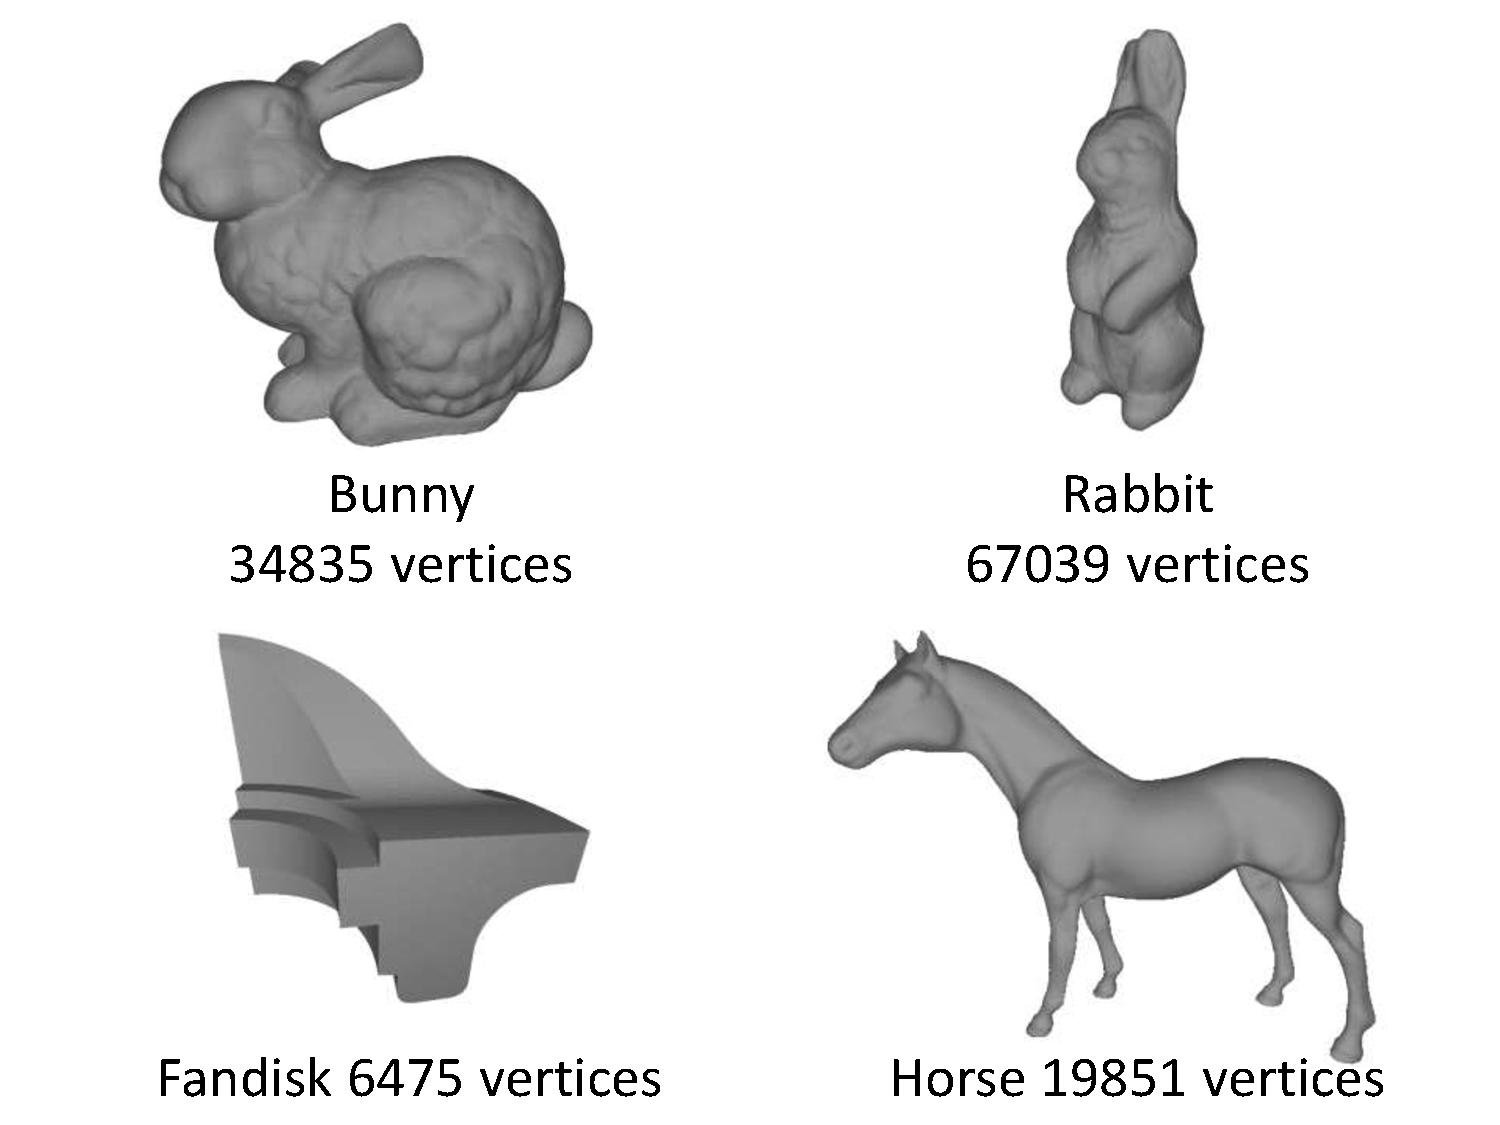
\includegraphics[width=4.0in]{images/experiments/test_data/modelsused}
\caption{Models used to assess the Plane-Tree compression algorithm.}
\label{fig:MODELSUSEDA}
\end{figure}

To test the Plane-Tree algorithm, several 3D objects commonly used within the literature were used to compare with known state of the art compression methods in terms of 3D mesh compression. The models used for testing are shown in figure \ref{fig:MODELSUSEDA}. These include: the bunny model with 34835 vertices, the rabbit model with 67039 vertices, the fandisk model with 6475 vertices and the horse model with 19851 vertices. \\

Several 3D reconstructions generated from the data set in appendix \ref{AppendixA} were used also to assess the Plane-Tree in compressing 3D reconstructions for storage and transmission. \\

